\chapter{Conclusion}\label{ch:conclusion}
Please recall that, the overarching goal of this thesis is three-fold Firstly, we aim to investigate whether a domain-specific measure is useful in MSA computation and develop a systematic methodology to leverage such a measure (Aim A). Secondly, we want to advance the state of the art of phylogeny estimation and closely related problems like species tree estimations (Aim B), and thirdly, we want to achieve this advancement through leveraging the multi-objective optimization framework (Aim C). In our case, the domain principally is phylogeny estimation and hence we introduce the concept of ‘phylogeny-awareness’. In this concluding chapter, we begin by summarizing our major contributions, by grouping them under our three broad aims, to highlight the notable findings that can be considered as the main takeaway of our thesis. Then we discuss possible directions for future extension and some of our ongoing works inspired by the central theme of this thesis.

\section{Summary of Findings}
Here we summarize the major contributions of this thesis by grouping them under our three overarching aims to highlight the notable findings that can be considered as the main takeaway of our thesis. 

\subsection{Develop a systematic methodology to leverage a domain-specific measure in MSA computation (Aim A)}
We introduced a phylogeny-aware multi-objective optimization approach to compute MSA with an ultimate goal to infer the phylogenetic tree from the resultant alignments. We studied and short-listed several objective functions widely used in the literature to compute MSA based on their efficacy. Moreover, we proposed some novel objective functions and investigate the efficacy thereof. We judged the potential capability of each objective function to yield better trees by employing domain knowledge as well as by applying statistical approaches on simulated datasets with the help of NSGA-III. We employed multiple linear regression to measure the degree of association between the individual objective functions and the quality of inferred phylogenetic tree (i.e., FN rate). Thus, we provide empirical justification to choose two bi-objective formulations based on two criteria: (a) the selected two objectives should be conflicting with each other (b) the selected objectives should exhibit relatively better correlation with the FN rate. 

To demonstrate the benefit of our identified bi-objective formulations, we performed extensive experimentation with biological rRNA datasets and BAliBASE 3.0 benchmark by executing NSGA-II and MOEA/D. We evaluated the generated solutions using generic alignment accuracy measures (e.g., SP-score, TP-score) as well as FN rate. We compare these solutions with the outputs of the state-of-the-art MSA methods to demonstrate the performance of our bi-objective formulations. We showed that both the bi-objective phylogeny-aware formulations can lead to phylogenetic trees with improved accuracy than that of the state-of-the-art MSA tools. From this finding, we hypothesized that, the use of domain specific measures can aid an MSA methods in other application domain as well.

\subsection{Advance the state of the art of phylogeny estimation leveraging the MO framework (Aim B, C)}
We delved into inferring better phylogenetic trees from MSAs by incorporating many application-aware objective functions through decomposition-based MO principles. In this direction, we developed the PMAO framework, which is based on PASTA, one of the most celebrated algorithms/tools in this regard. We evaluated the PMAO framework and examined its capability to yield high-quality tress by experimenting on the widely-used BAliBASE 3.0 benchmark. The PMAO framework, like other multi-objective algorithms, outputs a good number of alternative solutions that are equivalent (usually referred to as the non-dominated solutions) in the context of the conflicting objectives considered in the MO framework. Some of these solutions may however be of relatively lower quality from the application perspective. To this end, we innovatively employed machine learning to help PMAO generate only five solutions encompassing at least one top quality solution. Furthermore, summarizing those five solutions to obtain a single one offered better accuracy over PASTA in most of the cases, although not as good as the overall PMAO best.

In the sequel, we presented MAMMLE, a framework through which we infuse the concept of MO application-awareness into MUSCLE by incorporating our identified four application-aware objectives within the iterative refinement phase thereof through an MO strategy. MAMMLE generates multiple alternative alignments and for each of them an ML tree is inferred. We took these multiple hypotheses into our advantage and developed an ensemble approach for producing a better phylogenetic tree. MAMMLE offered a significant improvement (upto 27\% in our experiments) in tree accuracy over MUSCLE. We implemented our overall approach for phylogeny estimation from unaligned sequences as a flexible framework whose components can potentially be modified, replaced or further refined by bioinformatics researchers and practitioners.

Finally, we formulated the task of species tree estimation by summarizing a set of given gene trees as MO optimization task by accumulating the optimization criterion of the state-of-the-art methods (e.g., ASTRAL, MP-EST, STELAR). To effective tackle the task, we presented an multi-objective optimization algorithm, namely, SNOGA. To design SNOGA, we modified the popular NSGA-II in a way that enables them to retain some dominated solutions, otherwise discarded, which potentially evolve into a highly accurate species tree at a later generation. Our experimental results on a collection of simulated datasets demonstrated that the multi-objective approach can lead us to a tree-space containing significantly better trees than the trees estimated by ASTRAL and MP-EST which are two of the most widely used methods. 


\section{Future Extensions}
We now discuss several ways of extending the research works presented in this thesis as follows.
\begin{itemize}
	\item In this thesis we relied on the MO optimization strategies relate to the most popular MO metaheuristics (e.g., NSGA-II, NSGA-III, MOEA/D). Principles introduced by the recently developed MO algorithms (e.g.,~\cite{8981871, 9047876, 9097242}) can be experimented to find out which one can give us the best performance.
	
	\item We focused on developing effective optimization approaches for phylogenetic analyses rather than improving the runtime. Howe ever it is possible to achieve enough speedup by utilizing advanced computing architectures (e.g., GPU, cluster, etc.) as well as efficient implementation of core MO operations (e.g., \cite{8255834, 7738460}). 
	
	\item The genetic operators (i.e., mutation and crossover) used in this thesis randomly modifies a solution. We can embed domain knowledge inside those operators so that they can make informed (as opposed to random) rearrangement in the provided solution.  
	
	\item The calculation of objective functions are computationally expensive. We can develop machine learning based meta-models or surrogate models to make a low-fidelity approximation of the objective functions. 
	 
	\item We employ simple ensemble methods summarizing methods (i.e., greedy consensus and quartet consistency) to get a single solution from our MO frameworks. Further research efforts can be invested to enhance the ensemble methods.

	\item Throughout this thesis, we used only maximum likelihood for estimating phylogenetic trees. Alternatively, phylogenetics could also be estimated using Bayesian methods to generate a distribution of trees which can aid in designing a novel ensemble approach to generate the single output tree. But this would heavily increase the overall runtime of the pipeline.
	
	\item In this thesis, we adopt the common assumption that the underlying evolutionary history follows a tree structure. However, several biological processes (i.e., horizontal gene transfer, recombination of lineages, etc) are best described when evolutionary relationship is represented as a network. As our MO framework naturally generates several hypotheses of the phylogeny, it is worth investigating the advantages of providing the final output as network-like complex evolutionary models.

	
%	\item To enable SNOGA processing large datasets within a reasonable time, we will improve the efficiency of objective evaluations. Moreover, we are adapting a popular decomposition based EMO algorithm, namely, MOEA/D~\cite{zhang2007moea}, to effectively solve this problem.
		
\end{itemize}

\section{Ongoing Works Inspired by this Thesis}
Currently, we are working on two real-world combinatorial optimization problems from two different domains but originated from the core motivation of this thesis. Although we consider them to be out of the scope of this thesis, still we would like to discuss them briefly along with some preliminary results to further demonstrate the usefulness of domain-specific measures along with MO strategies in practical problems. 

\subsection{Find Optimal Base Locations for the Rapid Response Vehicles Providing Emergency Medical Service}
In many cities around the world, local authorities or charity organizations maintain a limited number of rapid response vehicles (RRVs) each carrying a healthcare team to provide from door to door emergency medical service to the citizens on demand~\cite{roislien2018comparing, van2019improving, benabdouallah2017comparison}. An RRV is usually constrained by the rule that it cannot go to a location beyond a certain travel distance or time from its assigned base location. It is very important to find the optimal base locations for all RRVs that maximize the summation of incidents served by each RRV (let us call it the actual coverage) from large historical data. It is expected that the optimal base locations will also perform reasonably well on future incidents. Now calculating actual travel distance/time using map query to know whether an incident can be covered by an RRV makes any optimization algorithm computationally intractable. So usually a simple distance measure scheme (e.g., Euclidean, Manhattan, etc.) is adopted and the number of covered incidents based on that scheme (let us call it as the approximate coverage) is used the single objective function to be maximized. But such a strategy may result in base locations which are not desirable considering the actual coverage.

To tackle the aforementioned challenge we advocate the use of the actual coverage as a domain-specific measure and find multiple simple objective functions exhibiting significant association to the domain-specific measure. So far we have experimented with the following bi-objective formulation.

\begin{enumerate}[label=$F_\arabic*$)]
	\item Maximize the approximate coverage as mentioned above
	\item Minimize the sum of the distances (Euclidean/Manhattan) of all covered incidents from the closest candidate base locations
\end{enumerate}

This MO formulation gives us a limited number of Pareto non-dominated solutions for which it is feasible to compute the actual coverage using map query and select the best solution. We show our preliminary results in Figure~\ref{fig:rrv-results} where we compare the best solutions generated by several usual single-objective metaheuristics/heuristics against the best solution among the Pareto solutions generated by NSGAII for real historical data from England (4110 emergency incidents) varying the number of RRVs. We see that the best solution offered by a simple application-aware MO formulation helps to attain around 700 more actual coverage than the best single-objective approach.

\begin{figure}[!htbp]
	\centering
	
	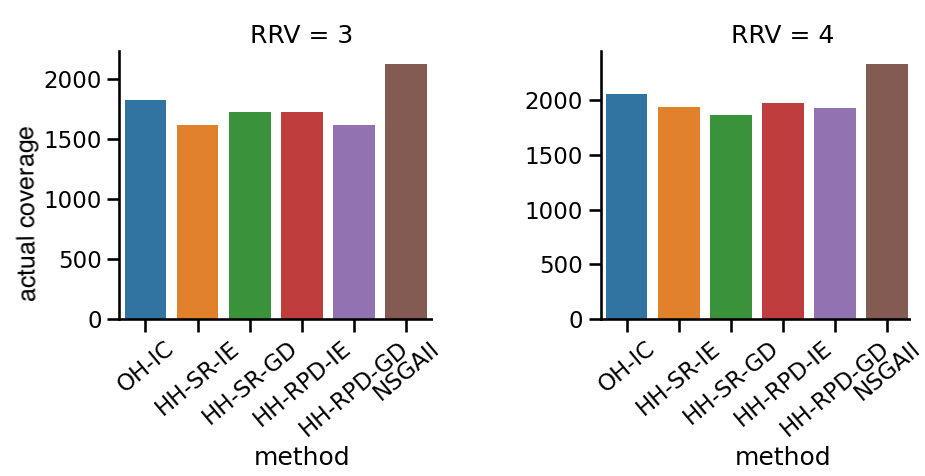
\includegraphics[width=0.8\textwidth]{Figure/rrv-results}
	\caption[Preliminary results on finding optimal base locations for RRVs]{Preliminary results on finding optimal base locations for RRVs. Here the x-axis shows different optimization methods and the y-axis shows the actual coverage calculated using real travel distance for the best solution generated by different approaches. OC-IC, HH-SR-IE, HH-SR-GD, HH-RPD-IE, HH-RPD-GD are different single-objective metaheuristics/heuristics. On the other hand, NSGAII optimizes the MO formulation detected using a domain-specific measure.}
	
	\label{fig:rrv-results}
	
\end{figure}

\subsection{Construct Efficient Bus Routes for Mass Evacuation }
Evacuation is one of the keys to saving human lives in times of natural and artificial calamities~\cite{alam2019development, alam2021shelter, alam2021dynamic}. Mass evacuation centrally arranged by the local authority through public buses has the potential to be a better alternative to ad-hoc evacuation in terms of minimizing the total evacuation time. Thus we get a fascinating optimization task to design an efficient set of bus routes that enable the evacuation of all inhabitants in the fewest possible time using the available buses. However, evacuation modeling is a complex task with a lot of uncertainty factors involved in the affected area. Given a candidate set of bus routes, usually, a micro-simulation tool is used to compute the total evacuation time (let us call it the actual evacuation time) which is very time-consuming and makes an optimization algorithm unrealistic. 

We are working to address the aforementioned challenge with the same spirit stemming from this thesis. To elaborate, we propose the use of the actual evacuation time as a domain-specific measure and find many simple application-orientated objectives. So far we have formulated the following five simple objective functions that have the potential to impact the actual evacuation time.

\begin{enumerate}[label=$F_\arabic*$)]
	\item Minimize the approximate evacuation time assuming there is no traffic congestion
	\item Minimize the sum of distances between a bus stop and its zone centroid
	\item Minimize the percentage of inhabitants that could not be evacuated
	\item Minimize the overlapping portion among different bus routes
	\item Minimize the sum of the length of all bus routes
\end{enumerate}

We have executed $\theta$-DEA~\cite{yuan2015new}, a popular MO metaheuristics for effectively tacking many objectives, on the 5-objective formulation and a 3-objective formulation to generate a limited number of Pareto solutions based on realistic data from a city of Canada (total 383 candidate bus stops, the city is divided into 56 zones) and then calculate the actual evacuation time using a simulator for each solution to see which ones can evacuate all the inhabitants with the minimum actual evacuation time. As a baseline, we also implement an ad-hoc heuristics that attempt to construct shorter bus routes one by one that can evacuate a larger portion of the total inhabitants until all inhabitants are evacuated. We run the heuristics a lot of times varying its parameters to generate a lot of solutions and finally calculate their actual evacuation time. actual We show a snapshot of our initial results in Figure~\ref{fig:halifax}. We notice that,  considering the lowest number of required routes (i.e., 24) application-aware MO formulation can save upto 3 hours of actual evacuation time.

\begin{figure}[!htbp]
	\centering
	
	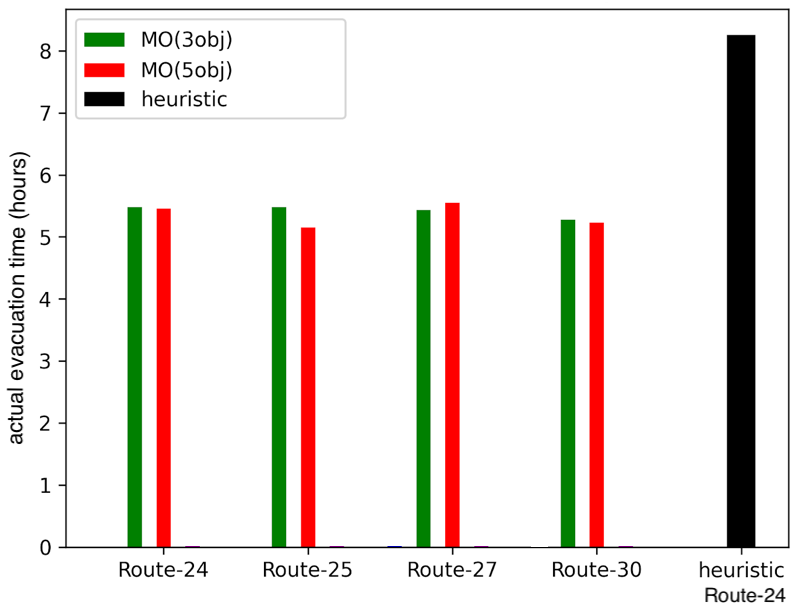
\includegraphics[width=0.6\textwidth]{Figure/halifax}
	\caption[Preliminary results on designing efficient bus routes for mass evacuation.]{Preliminary results on designing efficient bus routes for mass evacuation. Here the x-axis shows different optimization methods and the y-axis shows the actual evacuation time calculated by a simulator for the best solution (i.e., can evacuate all inhabitants within the minimum actual evacuation time) generated by different approaches. MO(5obj) and MO(3obj) are obtained by running $\theta$-DEA algorithm on the 5-objective formulation and a 3-objective formulation respectively varying number of required routes. On the other hand, heuristic is an ad-hoc heuristics designed to construct shorter bus routes one by one that can evacuate a larger portion of the total inhabitants.}
	
	\label{fig:halifax}
\end{figure}
%
%
%\section{Future Direction}
%
%In this study, we focus on developing an effective optimization approach to solve TNDP. However we do not consider its efficiency. The \textit{effectiveness} of an optimization algorithm refers to the quality of the solutions found or its robustness in finding desired solutions. The \textit{efficiency} characterizes the runtime behavior of the optimization algorithm. Along with efficiency, some other issues need to be considered for enhancing our current contribution. They are described as follows:
%
%\begin{itemize}
%	\item 	As the size and complexity of problem instances increase, the running time of any population based algorithm for solving TNDP like ours become unacceptable. The computational bottleneck is the time required to evaluate the objective functions of a solution. In future we can implement parallel models of MaOEAs to distribute the computational workload among multiple execution units.
%	
%	\item In this study we generate a fixed set of well-distributed reference points to guide the search directions of MaOEAs. If we can devise a generic way to integrate transport planners' preference in terms of a small set of objective vectors, we can reduce search directions as well as running time substantially. 
%	 
%	\item Currently our framework generates a set of alternative solutions for transport planners. To assist transport planners in choosing the ultimate solution, we can integrate Multi Criteria Decision Making (MCDM) methods into our framework for reducing the number of alternative solutions to a manageable size.
%	
%	\item At present we follow the common assumption that travel time and waiting time are independent of congestion effect. We can investigate the ways to integrate this effect into our evaluation model.
%	
%	\item We can refine our theoretical model by consulting transport planners and determine the applicability of our MaOEAs to real-world problems. We can also investigate how our problem-solving techniques can be integrated into commercial software toolkits such as VISUM, Emme/3.
%\end{itemize}
%
%\begin{figure}[h]
%	\centering
%	\begin{subfigure}[b]{0.4 \textwidth}
%		\includegraphics[width=\linewidth]{Figure/visum.jpg}
%		\caption{VISUM} \label{fig:visum}
%	\end{subfigure}
%	\hspace*{0.6cm} % separation between the subfigures
%	\begin{subfigure}[b]{0.5\textwidth}
%		\includegraphics[width=\linewidth]{Figure/emme.jpg}
%		\caption{Emme/3} \label{fig:emme}
%	\end{subfigure}
%	\caption{Commercial transport planning softwares.} \label{fig:transport_software}
%\end{figure}
